\chapter{Программная реализация информационной системы «Corpic» для обмена сообщениями}

Спроектированная в предыдущей главе архитектура, а также подходы и концепции использованы для реализации раннего прототипа информационной системы «Мессенджер», который содержит основной функционал, включающий себя регистрацию, авторизацию, текстовую коммуникацию в личных сообщениях, создание организаций, управление организацией, текстовая коммуникация внутри организаций, настройка и редактирование профиля.

\section{Реализация инфраструктурного серверного модуля, обеспечивающего работу с WebSocket подключениями и сообщениями}

Модуль «ws» отвечает за хранение WebSocket подключений, отправку сообщений пользователям, определяет интерфейс сообщения и ошибок (листинг \ref{ls:wsmodule}).

\begin{lstlisting}[caption={Модуль работы с WebSocket подключениями}, label={ls:wsmodule}]
@Module({
  imports: [],
  providers: [WsService],
  exports: [WsService],
})
export class WsModule {}
\end{lstlisting}

Сервис модуля хранит все текущие подключения в объекте ключ-значения, где ключом является идентификатор пользователя, а значением массив подключений. Также в сервисе реализованы методы отправки сообщения и удаления подключения (листинг \ref{ls:wsservice}).

\begin{lstlisting}[caption={Примеры методов сервиса WsService}, label={ls:wsservice}]
public getConnectedWebSocketsByUserId(userId: string): WsStateValueInterface[] | undefined {
  const webSockets = this.webSocketState.get(userId);
  return webSockets;
}

public setConnectedWebSocketByUserId(userId: string, webSocket: WebSocketEntity): string {
  if (!this.webSocketState.has(userId)) {
    this.webSocketState.set(userId, []);
  }

  const id = randomUUID();

  this.webSocketState.get(userId).push({ id, client: webSocket });

  return id;
}
\end{lstlisting}

В модуле реализован фильтр, обрабатывающий исключения. Перехваченное исключение записываться в серверный лог, после чего в случае, если оно предназначено к отправке на клиент, выполняется отправка сообщения с ошибкой (листинг \ref{ls:wsfilter}).

\begin{lstlisting}[caption={Фильтр обрабатывающий WebSocket исключения}, label={ls:wsfilter}]
@Catch()
export class WsFilterException extends BaseWsExceptionFilter {
  private readonly logger = new Logger(WsFilterException.name);

  catch(exception: { error: WsFormatExceptionInterface, message: string, eventName: string }, host: ArgumentsHost) {
    const client = host.switchToWs().getClient<WebSocketEntity>();

    this.logger.log(JSON.stringify(exception));

    if (exception.eventName && exception.error) {
      client.send(pack({
        event: exception.eventName,
        response: {
          status: false,
          errors: exception.error.message ?? exception.error,
        },
      }));

      if (exception.error.isCloseWs && exception.error.code) {
        client.close(exception.error.code);
      }
    }
  }
}
\end{lstlisting}

Написанный с помощью библиотеки RxJS, которая реализует парадигму реактивного программирования, перехватчик, добавляет к каждому перехваченному запросу контекст выполнения, который собирается из метаданных шлюза (листинг \ref{ls:wsinterceptor}).

\begin{lstlisting}[caption={Перехватчик добавляющий контекст выполнения к WebSocket запросу}, label={ls:wsinterceptor}]
@Injectable()
export class WsFormatInterceptor implements NestInterceptor {
  intercept(context: ExecutionContext, next: CallHandler): Observable<unknown> {
    const eventName = Reflect.getMetadata(
      'ws-message',
      (context.switchToWs() as unknown as { handler: unknown }).handler,
    );

    return next.handle().pipe(map((data: WsResponse<unknown>) => ({
      event: eventName,
      response: {
        status: true,
        key: data.key,
        data: data.data,
      },
    })), catchError((err: { error: WsFormatExceptionInterface, message: string, eventName: string }) => {
      err.eventName = eventName;
      return throwError(() => err);
    }));
  }
}
\end{lstlisting}

\section{Реализация серверного модуля, обеспечивающего аутентификацию пользователей}

Модуль аутентификации обеспечивает аутентификацию пользователей, защиту маршрутов всех шлюзов, определяет методы регистрации и авторизации (листинг \ref{ls:authmodule}). В зависимостях модуль требует модуль пользователей, JWT модуль, модуль работы с WebSocket, описанный ранее. Из модуля экспортируется охранник, обеспечивающий защиту Gateway маршрутов.

\begin{lstlisting}[caption={Модуль аутентификации}, label={ls:authmodule}]
@Module({
  imports: [
    MongooseModule.forFeature([
      {
        name: Session.name,
        schema: SessionSchema,
      },
    ]),
    JwtModule,
    WsModule,
    UsersModule,
  ],
  controllers: [
    AuthenticationController,
  ],
  providers: [
    AuthenticationGateway,
    AuthWsJwtGuard,
    AuthenticationService,
  ],
  exports: [
    AuthWsJwtGuard,
  ],
})
export class AuthenticationModule {}
\end{lstlisting}

Функциональность Gateway модуля аутентификации расширяется пятью декораторами, перехватчик \verb|WsFormatInterceptor| привязывает контекст выполнения к запросу, фильтр \verb|WsFilterException| перехватывает ошибку, охранник \verb|AuthWsJwtGuard| обеспечивает защиту маршрутов, труба \verb|WsValidationPipe| обеспечивает валидацию входных параметров на основе описанных моделей, декоратор \verb|WebSocketGateway| определяет объявленный класс как шлюз (листинг \ref{ls:authgateway}).

\begin{lstlisting}[caption={Определение шлюза модуля аутентификации}, label={ls:authgateway}]
@UseInterceptors(WsFormatInterceptor)
@UseFilters(WsFilterException)
@UseGuards(AuthWsJwtGuard)
@UsePipes(new WsValidationPipe({ skipMissingProperties: true, validationError: { target: false, value: false } }))
@WebSocketGateway(8080, { cors: true })
export class AuthenticationGateway implements OnGatewayDisconnect {...}
\end{lstlisting}

Для примера, рассмотрим маршруты авторизации и аутентификации пользователя (листинг \ref{ls:authgatewaylogin}). Маршрут авторизации в качестве тела запроса принимает модель \verb|AuthLoginDto| (листинг \ref{ls:authgatewaylogindto}), которая валидируется на основе модели, также в метод инжектируются данные клиента \verb|WebSocketEntity| (листинг \ref{ls:authgatewayloginclient}).

\begin{lstlisting}[caption={Определение маршрута входа}, label={ls:authgatewaylogin}]
@Public()
@MessageMetaData('auth-login')
@SubscribeMessage('auth-login')
async login(
  @MessageBody() body: AuthLoginDto,
@ConnectedSocket() client: WebSocketEntity,
) {
  const tokenAccess = await this.authService
    .createSession(body.email, body.password, client.remoteAddress);

  return {
    data: tokenAccess,
  };
}
\end{lstlisting}

\begin{lstlisting}[caption={Модель входных данных маршрута входа}, label={ls:authgatewaylogindto}]
export class AuthLoginDto {
  @IsString()
  @IsEmail()
  @IsNotEmpty()
    email: string;

  @IsString()
  @IsNotEmpty()
  @MinLength(6)
  @MaxLength(32)
    password: string;
}
\end{lstlisting}

\begin{lstlisting}[caption={Модель данных клиента}, label={ls:authgatewayloginclient}]
export class WebSocketEntity extends WebSocket {
  public botId?: string;

  public userId?: string;

  public socketId?: string;

  public tokenAccess?: string;

  public remoteAddress: string;
}
\end{lstlisting}

Внутри маршрута вызывается метод \verb|createSession| из сервиса \verb|AuthenticationService| (листинг \ref{ls:authcreatesession}). Внутри метода происходит попытка найти пользователя с переданной почтой, если пользователь найден, полученный пароль хэшируется и сравнивается с хэшом из базы данных. В случае, если пароли равны, создается JWT токен, в базу данных записывается новая сессия, токен возвращается клиенту.

\begin{lstlisting}[caption={Метод создания пользовательской сессии}, label={ls:authcreatesession}]
async createSession(email: string, password: string, ip: string): Promise<string> {
  const user = await this.validatingPassword(email, password);

  const payload = { userId: user._id.toString() };
  const tokenAccess = await this.jwtService.signAsync(payload, {
    secret: this.configService.get<string>('TOKEN_ACCESS_SECRET'),
    expiresIn: this.configService.get<string>('TOKEN_ACCESS_EXPIRATION'),
  });

  await this.SessionModel.create({
    userId: user._id.toString(),
    token: tokenAccess,
    lastIp: ip,
    lastActivityDateTime: new Date(),
  });

  return tokenAccess;
}
\end{lstlisting}

В маршруте аутентификации на вход принимается JWT токен доступа, подпись полученного токена проверяется, корректность сессии проверяется по базе данных, текущее соединение помечается как аутентифицированное, соединение добавляется в список соединений пользователя в модуле WebSocket, клиенту возвращается ID пользователя (листинг \ref{ls:authroute}). Процесс получения токена доступа и последующей аутентификации с помощью него показан в виде диаграммы последовательности на рисунке \ref{fig:auth}.

\begin{lstlisting}[caption={Определение маршрута аутентификации}, label={ls:authroute}]
@Public()
@MessageMetaData('auth')
@SubscribeMessage('auth')
async authHandler(
  @MessageBody() tokenAccess: string,
@ConnectedSocket() client: WebSocketEntity,
) {
  await this.authService.setTokenAccessToConnection(client, tokenAccess);

  return {
    data: client.userId,
  };
}
\end{lstlisting}

\begin{figure}[H]
\begin{center}
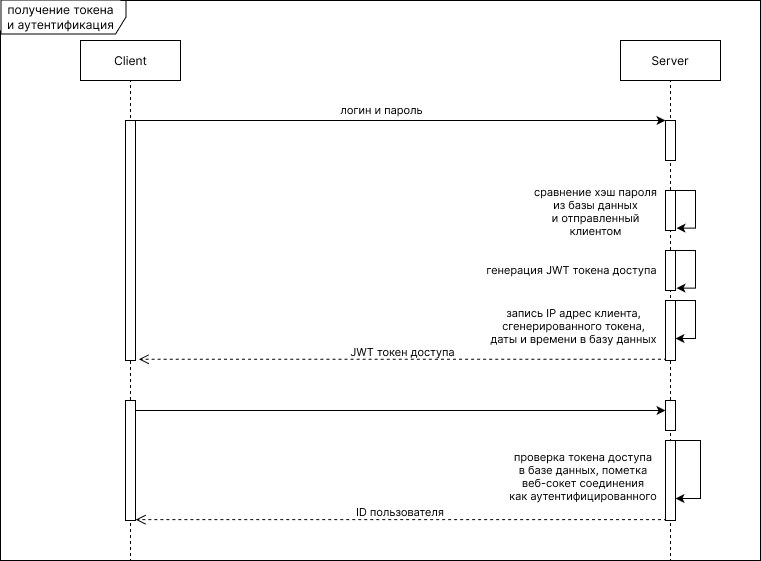
\includegraphics[width=1.0\hsize]{fig/auth.png}\\[2mm]
\caption{Процесс получения токена и аутентификации}\label{fig:auth}
\end{center}
\end{figure}

Помимо прочего, внутри модуля определяется охранник, защищающий маршруты от несанкционированного доступа. Внутри охранника, проверяется, что если маршрут помечен декоратором \verb|@Public|, то доступ к нему всегда открыт, иначе, доступ разрешен только в том случае, если соединение помечено как авторизованное (листинг \ref{ls:authguard}).

\begin{lstlisting}[caption={Охранник, защищающий маршруты от несанкционированного доступа}, label={ls:authguard}]
@Injectable()
export class AuthWsJwtGuard implements CanActivate {
  constructor(
    private readonly reflector: Reflector,
  ) {}

  async canActivate(context: ExecutionContext): Promise<boolean> {
    const client = context.switchToWs().getClient<WebSocketEntity>();
    const isPublic = this.reflector.getAllAndOverride<boolean>(IS_PUBLIC_KEY, [
      context.getHandler(),
      context.getClass(),
    ]);

    if (isPublic) {
      return true;
    }

    if (client.tokenAccess) {
      return true;
    }

    throw new WsFormatException({
      code: 3401,
      message: 'Token access is invalid',
    });
  }
}
\end{lstlisting}

\section{Реализация серверного модуля, обеспечивающего работу с чатами}

Функциональность Gateway модуля, обеспечивающего работу с чатами, расширяется пятью декораторами, которые уже были описаны ранее (листинг \ref{ls:chatsmodule}).

\begin{lstlisting}[caption={Определение шлюза модуля, обеспечивающего работу с чатами}, label={ls:chatsmodule}]
@UseInterceptors(WsFormatInterceptor)
@UseFilters(WsFilterException)
@UseGuards(AuthWsJwtGuard)
@UsePipes(WsValidationPipe)
@WebSocketGateway(8080, { cors: true })
export class ChatsGateway {}
\end{lstlisting}

В качестве примера, рассмотрим маршрут, который обеспечивает ленивую загрузку списка чатов пользователя (листинг \ref{ls:chatsget}). На вход маршрута поступает модель, в которой указан номер страницы пагинации, количество записей, которое нужно вернуть и нужно ли возвращать вложенные в модель объекты.

\begin{lstlisting}[caption={Определение шлюза модуля, обеспечивающего работу с чатами}, label={ls:chatsget}]
@UseInterceptors(ChatsApiFormattingInterceptor)
@MessageMetaData('chats-get')
@SubscribeMessage('chats-get')
async onGetChatsHandler(
  @MessageBody() body: GetChatsDto,
@ConnectedSocket() client: WebSocketEntity,
): Promise<WsResponse<{ chats: ChatDocument[], nextCursor?: number, prevCursor?: number }>> {
  const chats = (await this.chatsService.findByMembers([client.userId], {}, {
    extended: true,
    skip: body.page * body.count,
    limit: body.count,
  }));

  const chatsCounts = await this.chatsService.countChatsByMembers([client.userId]);

  const nextCursor = (chatsCounts - (body.page + 1) * body.count) > 0 ? body.page + 1 : undefined;

  return {
    data: {
      chats,
      nextCursor,
      prevCursor: body.page > 0 ? body.page - 1 : undefined,
    },
    meta: {
      currentUserId: client.userId,
    },
  };
}
\end{lstlisting}

Внутри маршрута вызывается метод сервиса \verb|findByMembers|, который ищет чаты, в которых участниками являются переданные пользователи, в данном случае, клиент вызывающий запрос (листинг \ref{ls:chatsfindbymembers}).

\begin{lstlisting}[caption={Метод поиска чатов по переданным участникам}, label={ls:chatsfindbymembers}]
async findByMembers(
  members: Array<string>,
  additional: FilterQuery<ChatDocument> = {},
  options = {
    extended: false,
    skip: 0,
    limit: 10,
  },
): Promise<ChatDocument[]> {
  const result = await ChatsService.cut<ChatDocument[]>(
    this.ChatModel.find({ ...additional, 'fullInfo.members.user': { $all: members } })
      .skip(options.skip)
      .limit(options.limit)
      .populate('lastMessage')
      .sort({ lastMessage: -1 }),
    options.extended,
  );

  return result;
}
\end{lstlisting}

Клиенту возвращается список чатов, значение следующей и предыдущей страницы. Перехватчик \verb|ChatsApiFormattingInterceptor| выполняет преобразование выходных данных, форматируя заголовок чата и последнее сообщение в чате.

\section{Реализация экрана просмотра списка личных чатов в веб-приложении}

Экран, содержащий список личных чатов пользователя является корневым маршрутов, он содержит в себе такие дочерние маршруты, как экран чата и экран просмотра информации о чате, все маршруты используют основной шаблон веб-приложения (листинг \ref{ls:routesMessages}).

\begin{lstlisting}[caption={Маршруты личных сообщений}, label={ls:routesMessages}]
export const routesMessages: RouteRecordRaw[] = [
  {
    path: '/messages',
    name: 'messages',
    component: () => import('@/views/Messages.vue'),
    meta: {
      layout: 'MainLayout',
    },
    children: [
      {
        path: 'direct/:chatId',
        name: 'direct',
        component: () => import('@/views/Chat.vue'),
        meta: {
          layout: 'MainLayout',
        },
        children: [
          {
            path: 'info',
            name: 'direct-info',
            component: () => import('@/views/chat/ChatInfo.vue'),
            meta: {
              layout: 'MainLayout',
            },
          },
        ],
      },
    ],
  },
];
\end{lstlisting}

Корневой компонент содержит шапку экрана, отображает список чатов или результат поиска в зависимости от состояния веб-приложения, отображает дочерний экран, в случае перехода на него. На мобильной версии, в случае перехода на дочерний экран, родительский экран удаляется из дерева компонентов, тем самым отображает дочерний компонент на полный экран (листинг \ref{ls:messagesview}).

\begin{lstlisting}[caption={Шаблон экрана личных сообщений}, label={ls:messagesview}]
<template>
  <div class="messages">
    <div v-if="isViewVisible" class="messenger-sidebar">
      <messages-header
        class="v-sidebar-header"
        :class="{ 'scroll': isSideBarScrolling }"
        @search-focus="searchStateChange(true)"
        @back-click="searchStateChange(false)"
        @search="onSearchDebounced"
      />

      <div class="sidebar-list">
        <v-scroll-dynamic
          v-if="!isSearchActive"
          :list-items-elements="getChatsResult?.pages"
          :container-ref="chatsContainerRef?.containerRef"
          :has-top-data="hasPreviousPage"
          :has-bottom-data="hasNextPage"
          ...
        >
          <chats-list
            v-if="!isSearchActive"
            ref="chatsContainerRef"
            :is-loading="isLoading"
            :pages="getChatsResult?.pages"
          />
        </v-scroll-dynamic>

        <n-scrollbar v-else class="sidebar-scrollbar">
          <messenger-search
            :searched-global-users="searchedGlobalUsers"
            :searched-global-chats="[]"
          />
        </n-scrollbar>
      </div>

      <new-chat-button />
      <div class="new-chat-popover" />
    </div>
    <nav-bar-mobile v-if="initialStore.isMobile && isViewVisible" />
    <router-view class="view-child" />
  </div>
</template>
\end{lstlisting}

Список чатов отображается внутри инфраструктурного компонента \verb|VScrollDynamic|, обеспечивающего ленивую загрузку и переиспользование UI элементов, повышает производительность. Компонент реализует двунаправленное добавление и удаление данных, при достижении нижней и верхней границы контейнера соответственно. Постраничная загрузка данных осуществляется при помощи библиотеки TanStack Query, выполняя запрос на описанный ранее серверный маршрут (листинги \ref{ls:getChatsResult}, \ref{ls:serviceGetChats}). Результат выполнения запроса на получение списка чатов показан на рисунке \ref{fig:web-app-get-chats-query}.

\begin{lstlisting}[caption={Использование TanStack Query для ленивой загрузки}, label={ls:getChatsResult}]
const queryClient = useQueryClient();
const {
  data: getChatsResult,
  error,
  isLoading,
  fetchNextPage,
  fetchPreviousPage,
  hasNextPage,
  hasPreviousPage,
  isFetching,
  isFetchingNextPage,
  isFetchingPreviousPage,
} = useInfiniteQuery(['get-chats'], getChats, {
  getNextPageParam: (lastPage) => lastPage.nextCursor,
  getPreviousPageParam: (firstPage) => firstPage.prevCursor,
});
\end{lstlisting}

\begin{lstlisting}[caption={Сервис запрашивающий список чатов}, label={ls:serviceGetChats}]
export const getChats = async ({ pageParam = 0 }): Promise<{ chats: ApiChat[],
  nextCursor?: number, prevCursor?: number }> => {
  const { ws } = useWebSocketStore();
  const result = await ws.emitPromised<{ chats: ApiChat[],
    nextCursor?: number, prevCursor?: number }>('chats-get', { count: 20, page: pageParam, extended: true });
  if (!result.status) {
    throw new Error(JSON.stringify(result.errors));
  }
  return result.data;
};
\end{lstlisting}

\begin{figure}[H]
\begin{center}
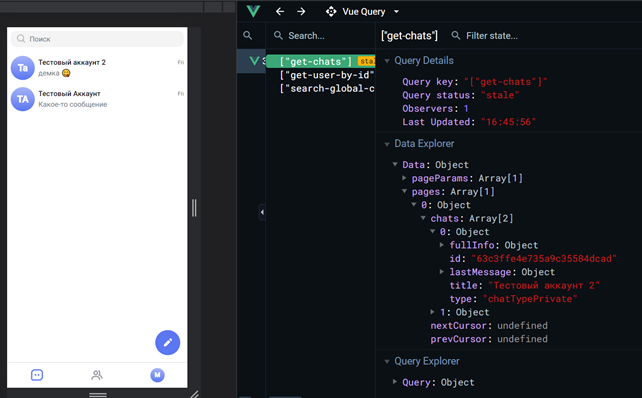
\includegraphics[width=1.0\hsize]{fig/web-app-get-chats-query.png}\\[2mm]
\caption{Результат выполнения запроса на получение списка чатов}\label{fig:web-app-get-chats-query}
\end{center}
\end{figure}

Для оптимизации поисковых запросов, используется концепция задержки запросов. Веб-приложение ожидает определенное количество времени (в данном случае 350 миллисекунд), пока пользователь не прекратит ввод, после чего выполняет запрос на сервер (листинг \ref{ls:searchGlobalChatsQuery}). Таким образом, запрос к серверу выполняется только после того, когда пользователь закончил вводить желаемый запрос. Результат выполнения поискового запроса показан на рисунке \ref{fig:web-app-search-query}.

\begin{lstlisting}[caption={Использование TanStack Query для запросов на сервер с задержкой}, label={ls:searchGlobalChatsQuery}]
const searchGlobalChatsQuery = ref('');
const { data: searchGlobalUsersResult } = useQuery([
  'search-global-chats',
  searchGlobalChatsQuery,
], () => searchGlobalUsers(searchGlobalChatsQuery.value));
const searchedGlobalUsers = computed(() => (
  searchGlobalUsersResult.value?.status ? searchGlobalUsersResult.value.data ?? [] : []
));

const onSearch = (query: string) => {
  if (query) {
    searchGlobalChatsQuery.value = query;
  } else {
    searchGlobalChatsQuery.value = '';
  }
};

const SEARCH_DURATION = 350;
const onSearchDebounced = useDebounce(onSearch, SEARCH_DURATION);
\end{lstlisting}

\begin{figure}[H]
\begin{center}
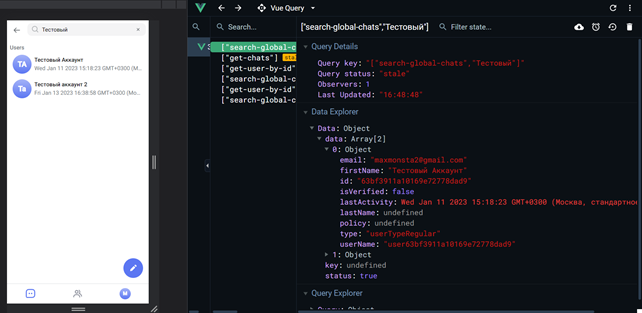
\includegraphics[width=1.0\hsize]{fig/web-app-search-query.png}\\[2mm]
\caption{Результат выполнения поискового запроса показан на рисунке}\label{fig:web-app-search-query}
\end{center}
\end{figure}

На экране чата отображается список сообщений чата, для их отображения используется концепция, аналогичная той, которая используется для отображения списка чатов.

На корневом уровне веб-приложения, запущены обработчики, прослушивающие сообщение с сервера. Для примера, рассмотрим обработчик поступления новых сообщений. Сервер отправляет сообщение на обработчик \verb|new-message| всем участникам чата, когда кто-то из участников создает новое сообщение.  В обработчике происходит инвалидация соответствующих запросов, которые запрашивают сообщения, после чего, состояние веб-приложения синхронизируется с сервером, реактивно отображая новые данные (листинг \ref{ls:messagesApiUpdaters}). Результат обновления состояния веб-приложения, после вызова обработчика показан на рисунке \ref{fig:web-app-ws-handler}.

\begin{lstlisting}[caption={Глобальный обработчик подписанный на WebSocket событие}, label={ls:messagesApiUpdaters}]
export const messagesApiUpdaters = (ws: WebSocketProvider, queryClient: QueryClient) => {
  ws.on('new-message', async () => {
    await queryClient.invalidateQueries(['get-messages']);
    await queryClient.invalidateQueries(['get-chats']);
  });
}; 
\end{lstlisting}

\begin{figure}[H]
\begin{center}
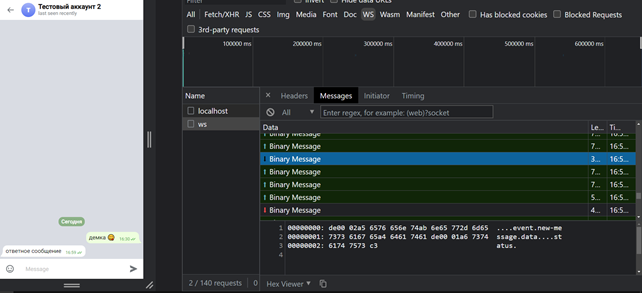
\includegraphics[width=1.0\hsize]{fig/web-app-ws-handler.png}\\[2mm]
\caption{Результат обновления состояния веб-приложения}\label{fig:web-app-ws-handler}
\end{center}
\end{figure}